\documentclass[a4paper,twocolumn]{article}


\usepackage[T1]{fontenc}
\usepackage[utf8]{inputenc}

\usepackage{graphicx}          % To handle figures
\usepackage{amsmath}           % Defines certain mathematical symbols

\addtolength{\topmargin}{-25mm}% Decrease the top margin by 25mm
\addtolength{\textheight}{25mm}% Increase the text height by the
                               % same amount

\begin{document}

\title{Bank filtering for sound compression}
\author{Baptiste Cavarec \\ 940321-T197 \and Hugo Lime\\
  920707-4635}
%\date{2000-10-10} % If you don't want todays date.

\maketitle


\begin{abstract}
In this report, we describe a simple implementation of bank filtering for sound compression. We explain how to construct theses filters and the effect of quantization of the decimated signals. We then provide a method to reduce the signal bitrate while preserving quality by choosing a proper bit allocation for the decimated signals.
\end{abstract}

\section{Introduction}
\label{sec:intro}

In this project, we intend to study the common problematic of data compression, in our case for sound signals. We have, as an input, a sound signal sampled at a 8 kHz frequency. In order to store and compress our signal, we need to implement an analysis filter bank. The one we decided to implement can be seen in Fig.~\ref{fig:analysis}. As one can also see in Fig.~\ref{fig:analysis}, we also compute quantization of our 3 signals obtained by the analysis. This is the core of our data storage issue, as we need to quantize in order to lower the signal's data rate. This obviously induces quantization noise and deteriorates the signal, we then have to find the best way to avoid the noise.

\begin{figure}[!ht]
  \begin{center}
    % Standard LaTeX can handle EPS files.
    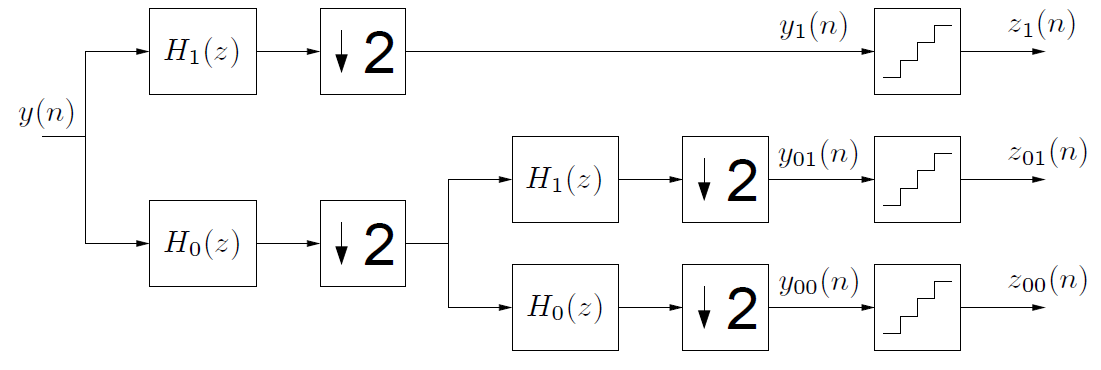
\includegraphics[width=0.83\columnwidth]{analysis.png}
    % If you instead use pdflatex to process the file, the
    % figures should be in PDF, JPG or PNG format.
  \end{center}
  \caption{Analysis filter bank followed by quantization.}
  \label{fig:analysis}
\end{figure}

Then, we use the synthesis filter bank presented in Fig.~\ref{fig:synthesis} in order to reconstruct the signal. Sec.~\ref{sec:reconstruction} will present the filters used and their impact on the signal.

\begin{figure}[!ht]
  \begin{center}
    % Standard LaTeX can handle EPS files.
    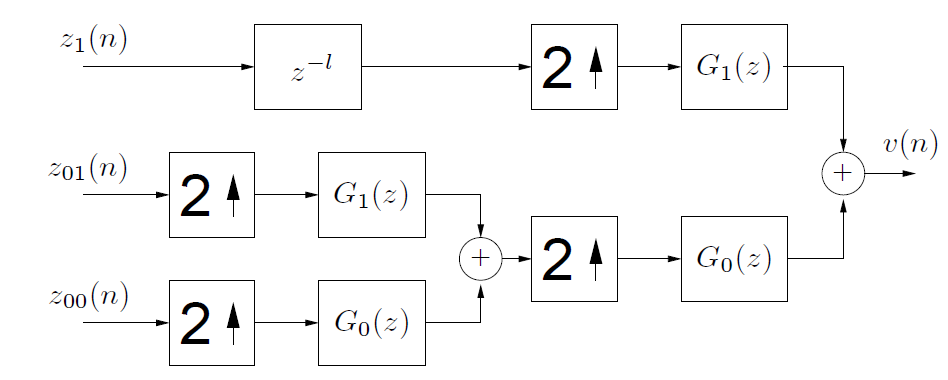
\includegraphics[width=0.83\columnwidth]{synthesys.PNG}
    % If you instead use pdflatex to process the file, the
    % figures should be in PDF, JPG or PNG format.
  \end{center}
  \caption{Synthesis filter bank.}
  \label{fig:synthesis}
\end{figure}

In order to evaluate the error introduced by the above mentioned quantization scheme, we need to introduce a measure of our quantization/reconstruction scheme efficiency as Sec.~\ref{sec:reconstruction} ensures perfect reconstruction, this measure would only seize the impact of the quantization on the compressed sound.
The measure we consider is called Signal to Quantification Noise Ratio (SQNR) and can be evaluated as in Eq.~\ref{eq:sqnr}. 
\begin{equation}
  \label{eq:sqnr}
  SQNR= \frac{E[y^2(n)]}{E[\left(y(n-L)-v(n)\right)^2]}
\end{equation}




\section{Bank filtering}
\label{sec:filtering}
\subsection{Filters}
\label{sec:reconstruction}
We presented in Sec.~\ref{sec:intro}, our structure is based on Analysis/Synthesis Filter Bank scheme (Fig.~\ref{fig:analysis} and Fig.~\ref{fig:synthesis}).
In order to ensure the reconstruction of our signal, we need to design the filters so that they respect Eq.~\ref{eq:filters1}, Eq.~\ref{eq:filters2} and Eq.~\ref{eq:condh0g0}.
\begin{equation}
  \label{eq:filters1}
H_1(z)=G_0(-z)
\end{equation}
\begin{equation}
\label{eq:filters2}
G_1(z)=-H_0(-z)		
\end{equation}
\begin{equation}
\label{eq:condh0g0}
G_0(z)H_0(z)-G_0(-z)H_0(-z)=2\cdot z^{-l}		
\end{equation}
 Moreover, in order to perform the synthesis scheme, we need to know the delay introduced by our Analysis/Synthesis bank. By using the formalism presented in Eq.~\ref{eq:g0h0} we ensure a delay $l=3$ for our "first order" filter bank, if Q is an order 2 polynomial in $z^{-1}$. If we want to ensure that Eq.~\ref{eq:condh0g0} is satisfied, we must have $Q(z)=-\frac{1}{16}+\frac{z^{-1}}{4}-\frac{z^{-2}}{16}$.
\begin{equation}
  \label{eq:g0h0}
G_0(z)H_0(z)=(1+z^{-1})^4Q(z)
\end{equation}
Given this, we choose:
\begin{equation}
 G_0(z)=\frac{1}{2}\left(1+z^{-1}\right)^2
\end{equation}
it then leads to 
\begin{equation}
H_0(z)=\frac{1}{8}\left(-1+2z^{-1}+6z^{-2}+2z^{-3}-z^{-4}\right)
\end{equation}
Hence, 
\begin{equation}
H_1(z)=\frac{1}{2}\left(1-z^{-1}\right)^2
\end{equation}
and
\begin{equation}
G_1(z)=-\frac{1}{8}\left(-1-2z^{-1}+6z^{-2}-2z^{-3}-z^{-4} \right)
\end{equation}

Fig.~\ref{fig:filters} shows the shape of these filters in frequency domain.


\begin{figure}[!ht]
  \begin{center}
    % Standard LaTeX can handle EPS files.
    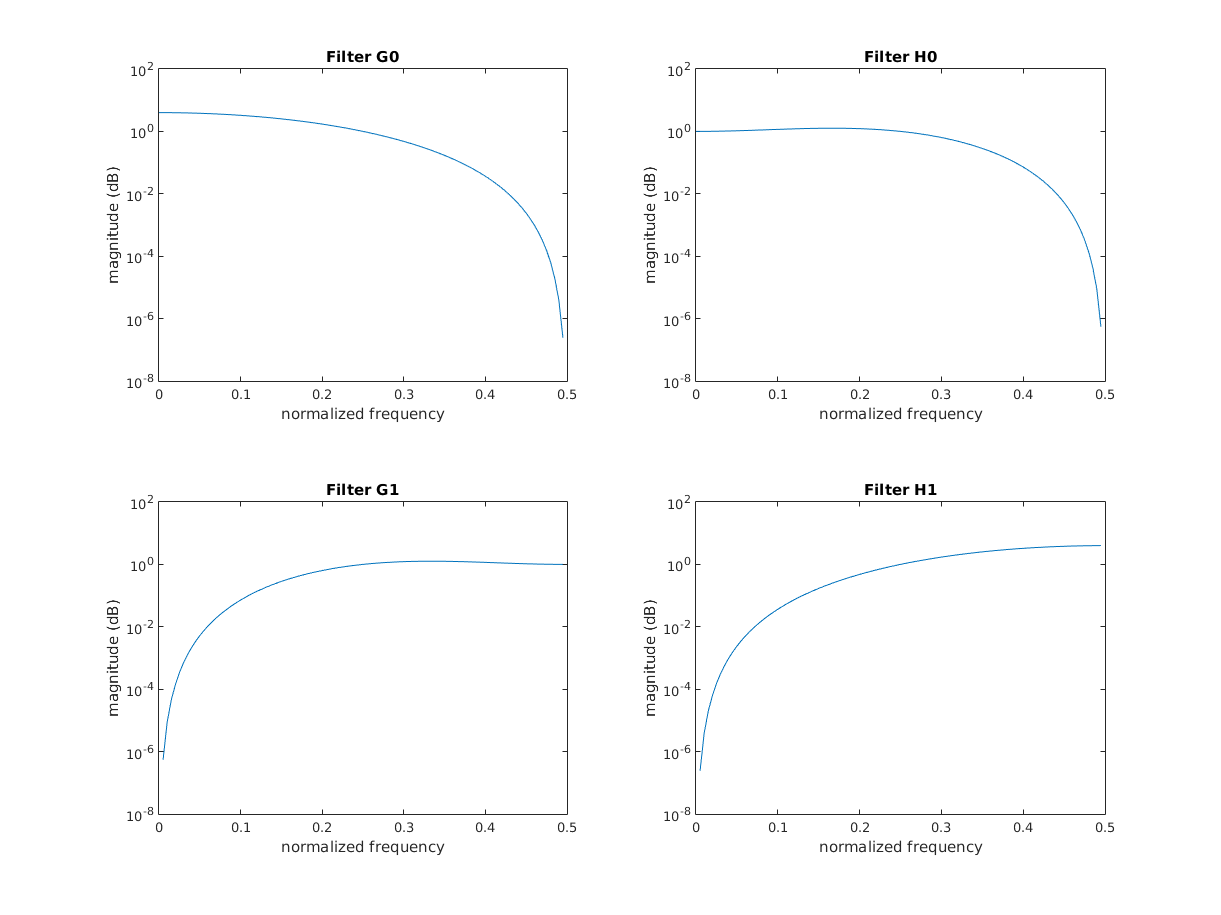
\includegraphics[width=1.1\columnwidth]{filters2.png}
    % If you instead use pdflatex to process the file, the
    % figures should be in PDF, JPG or PNG format.
  \end{center}
  \caption{Frequency response of the filters used in our Analsys/Synthesis scheme}
  \label{fig:filters}
\end{figure}


Given this, we will ensure in Sec.~\ref{sec:numreconstruction} that these filters perform perfect reconstruction.


\subsection{Total delay of the system}
As one can see in Sec.~\ref{sec:reconstruction}, we introduced a delay by implementing these filters. The delay created by the "first order" Analysis/Synthesis scheme is given and is $l=3$. Therefore, we implemented an artificial delay of $3$ on $z{1}(n)$ to compensate the delay induced by the nested Analysis/Synthesis scheme on the other branch. These delays are done on downsampled signals and result in a $2 \cdot 3$ delay after upsampling. Moreover, the external Analysis/Synthesis also created a delay of 3 leading the whole delay to be $L=9$.

\subsection{Perfect reconstruction}
\label{sec:numreconstruction}
In order to check our filter bank implementation, we measured the avarge error between the input signal and the delayed output signal.
\begin{equation}
error=\frac{1}{N}\sum_{n=1}^{N-1}|v(n+9)-y(n)|^{2}
\end{equation}
with $N$ being the total number of samples. As expected by our choice of filter, we obtain a null error meaning that we have perfect reconstruction of the signal.


\section{Decimated signals}
\label{sec:decimated}

\subsection{Relation with the input signal}
The decimated signals are linked to the input signal as they represent a certain band of its frequencies. If we study the filters $H_{0}$ and $H_{1}$, we can consider them to be respectively a low-pass and high-pass filter. Graphical study with Fig.~\ref{fig:filters} shows that the $-3dB$ bandwidth of $H_{0}$ is approximately [0,0.3] and the one of $H_{1}$ is [0.3,0.5]. 

To simplify, we can consider them to be ideal filters with bandwidths [0,0.25] and [0.25,0.5] so that there is no aliasing. We can therefore consider that the decimated signals would represent the spectrum of the signal in theses bands. Fig.~\ref{fig:spect} shows how the spectrum of the input signal (here file "thank.wav") is split in three with these filters.

\begin{figure}[!ht]
  \begin{center}
    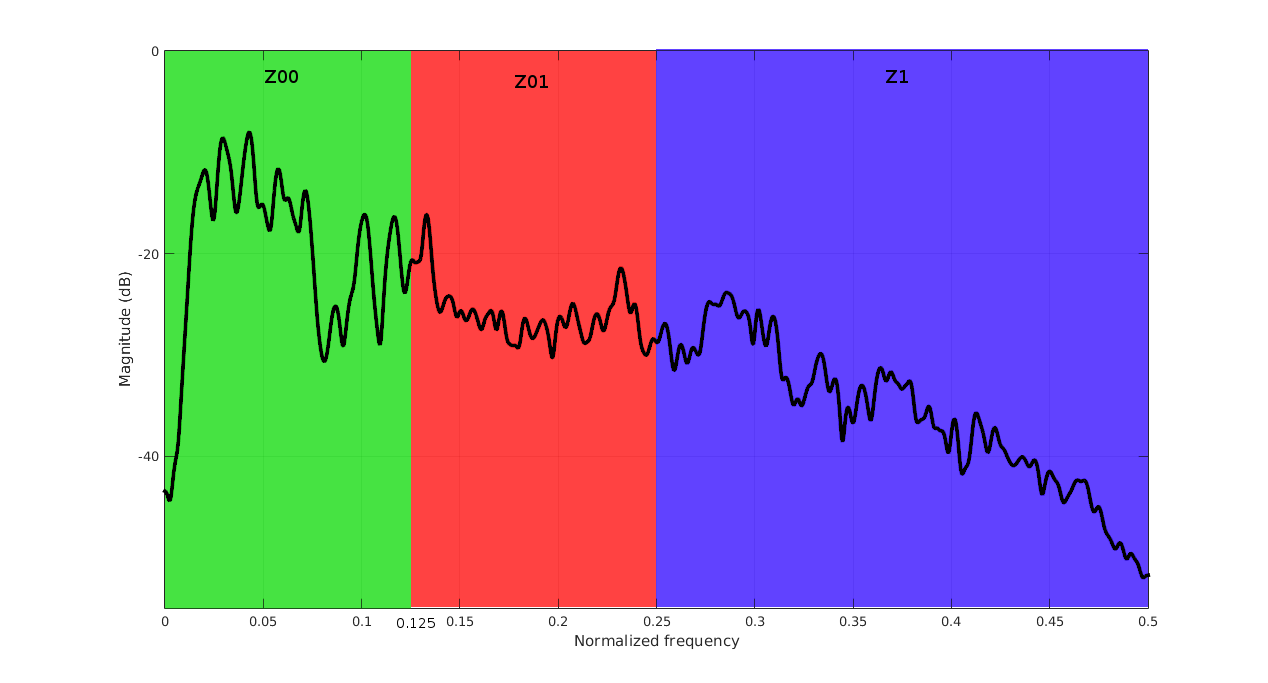
\includegraphics[width=1.1\columnwidth]{Thank_spectrum5.png}
  \end{center}
  \caption{Spectrum splitting of input signal}
  \label{fig:spect}
\end{figure}
As one may have expected, when we listen to the intermediate signal we can notice that the high band signal y1 on Fig.~\ref{fig:analysis} is mostly composed of high pitch of the signal and the low band signal y0 is composed of the low frequencies of the signal. When considering the second order of our Analysis scheme, we can hear that y00 is very deep and y01 is quite hard to caracterize as it is "high frequencies" of the low band.

\subsection{Effects of the downsampling on the signal}
The downsampling results on the spreading of the spectrum over a broader part of our normalized frequency domain. For instance, the $[0;\frac{1}{2}]$ domain is mapped onto $[0;1]$ when we downsample of a factor 2 as for the considered application. Then aliasing occurs, adding the parts that are over [-1/2;1/2] periodically as one can see on Eq.~\ref{eq:downsampling}. 
\begin{equation}
  \label{eq:downsampling}
y(\nu)=\frac{1}{2}\sum X\left(\frac{\nu-k}{2}\right)
\end{equation}
This phenomenon can be seen in Fig.~\ref{fig:downsampling} we can clearly see that the global behaviour of the downsampled signal looks like the $[0,0.25]$ part of the original one but it is not totally alike, due to aliasing. As expected from the previous curve, the downsample signal sounds "deeper" than the original one, as we have more low frequencies.

\begin{figure}[!ht]
  \begin{center}
    % Standard LaTeX can handle EPS files.
    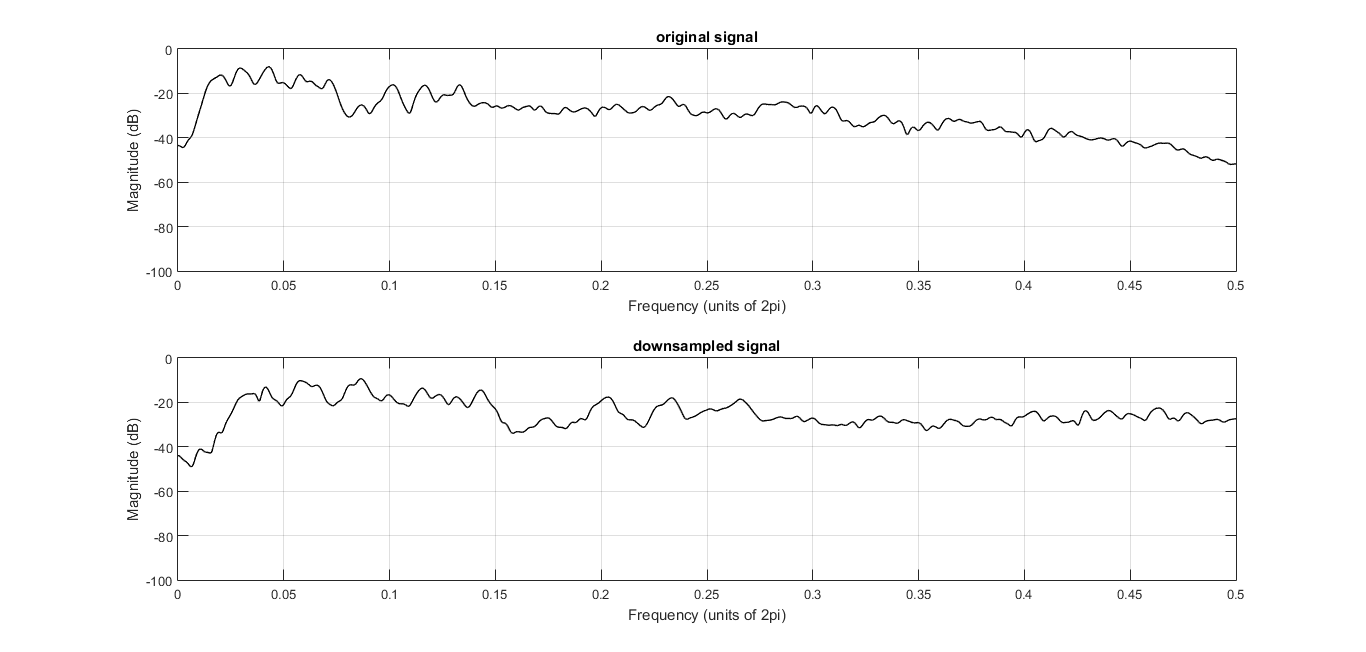
\includegraphics[width=1.1\columnwidth]{downsampling.png}
    % If you instead use pdflatex to process the file, the
    % figures should be in PDF, JPG or PNG format.
  \end{center}
  \caption{Effects of the downsampling on the thank.wav signal}
  \label{fig:downsampling}
\end{figure}





\section{Quantization}
\label{sec:quantization}

\subsection{Effects of quantization}
\label{sec:quantizationeffect}
In order to store or transmit our signal we need to assign a certain number of bits to represent the value of each sample. A greater number of bits would allow to represent more values and thus allowing higher fidelity but would also require larger memory or bitrate. Fig.~\ref{fig:quant} shows that a $32~kbit/s$ bitrate would give a SQNR of $12.87~dB$ for the file "thank.wav".

\begin{figure}[!ht]
  \begin{center}
    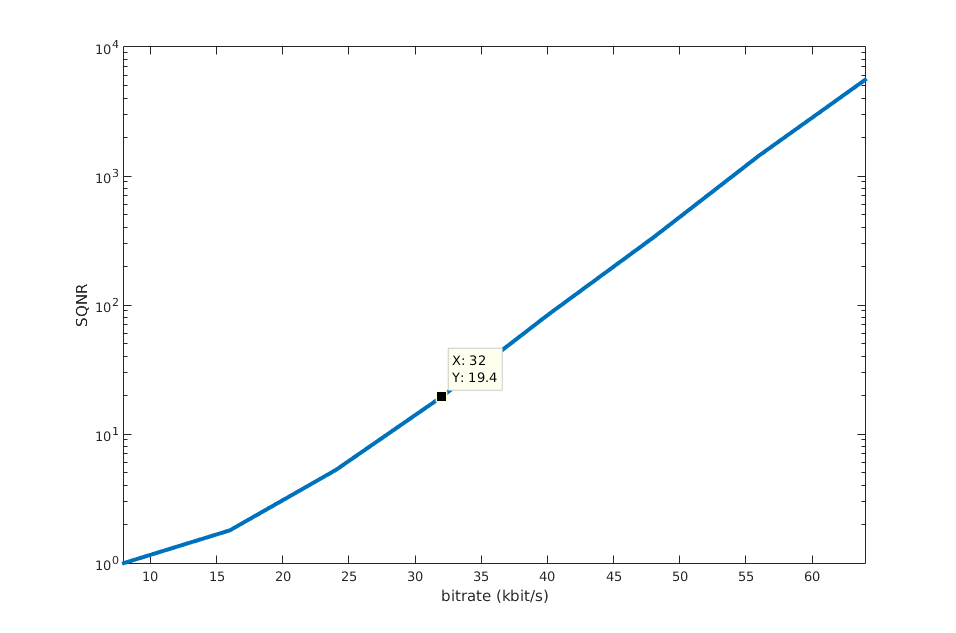
\includegraphics[width=1.1\columnwidth]{quantization.png}
  \end{center}
  \caption{SQNR for different bitrates without filter bank}
  \label{fig:quant}
\end{figure}

\subsection{Quantization in filter banks}
In order to improve this result, we can use our filter bank by transmitting the decimated signals $z_{1}(n)$, $z_{01}(n)$ and $z_{00}(n)$ instead of $y(n)$. We can allocate different numbers of bits for the decimated signals which allows to have higher fidelity for some frequencies which are more important.
Lets define $b_{1}$, $b_{01}$ and $b_{00}$ as the number of bits allocated to represents samples of the signals $z_{1}(n)$, $z_{01}(n)$ and $z_{00}(n)$.
Given the fact that the rate of $z_{1}(n)$ is half the one of $y(n)$ and that the rate of $z_{01}(n)$ and $z_{00}(n)$ is one fourth the one of $y(n)$, the total bitrate is given by Eq. \ref{eq:rate}.
\begin{equation}
  \label{eq:rate}
  bitrate = 8(\frac{b_{1}}{2}+\frac{b_{01}+b_{00}}{4})~kbit/s
\end{equation}


\subsection{Bit allocation}
If we want to improve the SQNR obtaine in Sec.~\ref{sec:quantizationeffect} for a $32~kbit/s$ transmition, Eq.~\ref{eq:rate} leads to equation \ref{eq:bit}
\begin{equation}
  \label{eq:bit}
  2b_{1}+b_{01}+b_{02}=16
\end{equation}
To obtain the best bit allocation, we tested all combinations. For the file "thank.wav", the best bit allocation is $b_{1}=3$, $b_{01}=4$ and $b_{00}=6$ giving a SQNR of $16.9~dB$.\\

However, when testing on the file "orinoccio.wav", the best bit allocation is $b_{1}=2$, $b_{01}=5$ and $b_{00}=7$ giving a SQNR of $20.3~dB$ instead of $9.6~dB$ without filter bank.\\

The best bit allocation thus depend on the sound signal. As we can see on Fig.~\ref{fig:spectrum}, The magnitude of the spectrum decrease with the frequency which explains why for both signals, the best allocation is to give more than half the bandwith to the low-frequencies. Moreover, for the "orinoccio.wav" signal, we can notice that the spectrum is very much concentrated around very low frequencies which explains why $b_{00}=7$.
\begin{figure}[!ht]
  \begin{center}
    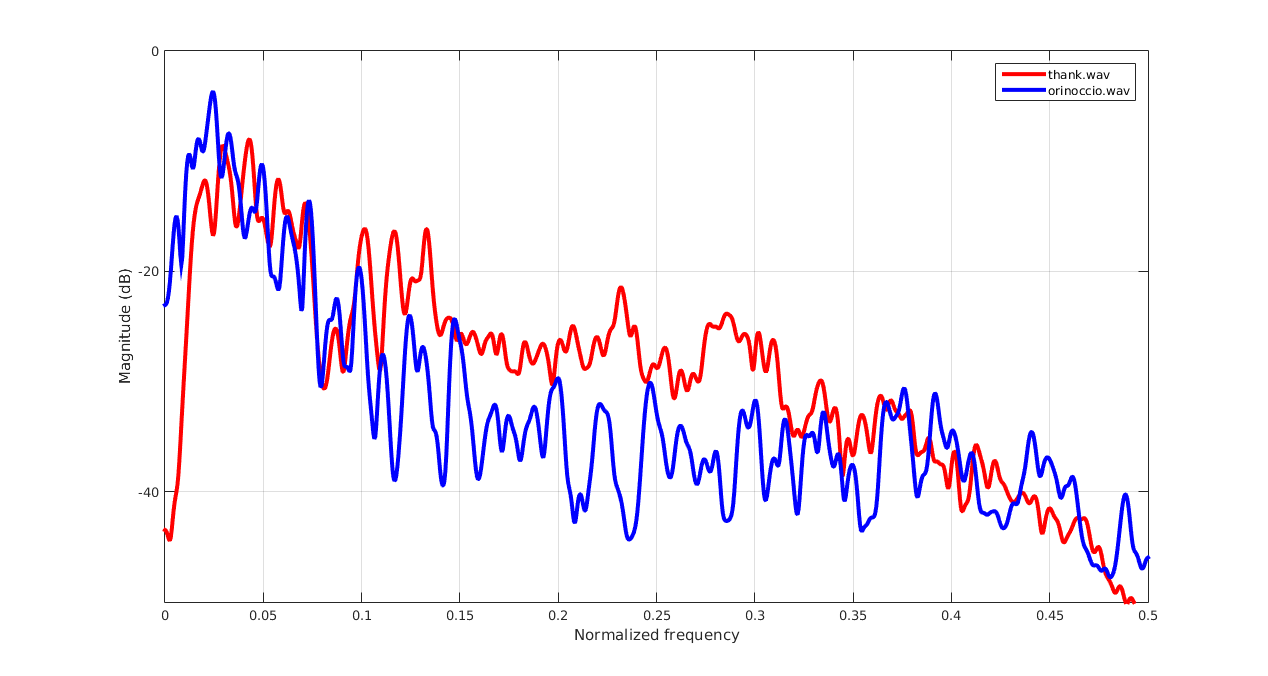
\includegraphics[width=1.1\columnwidth]{spectrum3.png}
  \end{center}
  \caption{Spectrum of input signals}
  \label{fig:spectrum}
\end{figure}
Therefore, it is also possible to devise a bit allocation only by analysing the signal spectrum but it will not be as good as testing all bit allocations.

\subsection{Perceived quality}
To measure the fidelity of the reconstucted signal, we have used the SNQR (Eq.~\ref{eq:sqnr}). Basicaly, it measures the error, sample by sample, between the recontructed signal ans the input signal. In order to determine if the SQNR is a good measure of the perceived distorsion we computed different configurations of bit repartition that lead to a different SQNR. We have heard that the higher the SQNR, the less audible the noise was, that was to be expected from the formula of the SQNR (Eq.~\ref{eq:sqnr}). During this experiment we also heard that two close SQNR can lead to a different "feeling" of the noise you hear, depending if the quantization noise is located more in the low frequency band or the high frequency ones. This leads us to say that even if SQNR is a good measure of the quantization noise, it is not really representative of the experience of the quality of a human user.


\section{Conclusions}
\label{sec:conclusions}

To conclude this study of bank filtering and sound compression, we can say that:
\begin{itemize}
\item We can devise filters to create filter banks with perfect reconstruction.
\item Quantization, which is necessary to store or transmit a signal, creates error in the reconstructed signal.
\item Allowing different number of bits to the decimated signal can greatly improve the SNQR. We described a method to obtain the best bit allocation.
\end{itemize}

We can also add that in order to improve the compression, a deeper study of how humans perceive a sound should be done. For example, it could be interesting to see if some frequencies are more important for a human hear and also how humans perceive two neighbouring frequencies.

\end{document}
